\documentclass[a4paper, 11pt]{article}
\usepackage{geometry}
\geometry{letterpaper, margin=1in}
\usepackage{amsmath}
\usepackage{amssymb}  
\usepackage{amsthm}
\usepackage{ulem} 
\usepackage{graphicx}
\usepackage{enumitem} 
\graphicspath{ {images/} }


\newtheorem*{theorem}{Theorem}

\begin{document}
%Header-Make sure you update this information!!!!
\noindent
\large\textbf{Complex Analysis: Day 17} \hfill \textbf{John Waczak} \\
\normalsize MTH 483 \hfill  Date: \today \\


\subsection*{Limsup} 
	\textbf{Def} let $a_n$ be a sequence of nonnegative real numbers. 
		\begin{itemize}
			\item If $\{a_n\}$ has a subsequence that is unbounded, we say
				\begin{equation*}
					\limsup_{n\rightarrow +\infty} a_n = + \infty
				\end{equation*}
			\item If $\{a_n\}$ is bounded, we define: 
				\begin{equation*}
					\limsup_{n\rightarrow +\infty} a_n 
				\end{equation*}
				to be the largest limit of any convergent subsequence of $\{a_n\}$
		\end{itemize}
		
	\noindent \textit{Examples} 
		\begin{itemize}
			\item $\limsup_{n\rightarrow+\infty}(1+\frac{1}{n}) = 1$ 
			\item $a_n = 4+(-1)^n = \{3, 5, 3, 5, ...\}$ thus $\limsup_{n\rightarrow+\infty} a_n = \lim_{n\rightarrow \infty}\{5,5,5,5,...\} = 5$. 
		\end{itemize}

	\noindent The \textbf{big-picture} goal is
		\begin{itemize}
			\item to show that functions defined by power series are holomorphic where they converge absolutely. 
			\item Conversely, if $f:\Omega\rightarrow\mathbb{C}$ is holomorphic and $c\in\Omega$, then there exists a disc $D_r(c)\subseteq \Omega$ on wich f is given by a power series. 
		\end{itemize} 
	


\subsection*{More on power series} 
	\begin{theorem}
		Let $\sum\limits_{n=0}^\infty a_n(z-c)^n$ be a power series where $a_n,c\in\mathbb{C}$. Then $\exists 0\leq R\leq +\infty$ such that:
			\begin{enumerate}[label=\alph*]
				\item If $|z-c|<R$ then the series converges absolutely 
				\item If $|z-c|>R$ the series diverges. 
			\end{enumerate} 
		
		
		
		Moreover, we have that $R=\frac{1}{L}$ where $L=\limsup_{n\rightarrow+\infty} |a_n|^{1/n}$ Interpret $\frac{1}{0} = +\infty$, $\frac{1}{+\infty} = 0$. 
	\end{theorem}	\pagebreak
	
	\begin{figure}[!hbt]
		\centering
		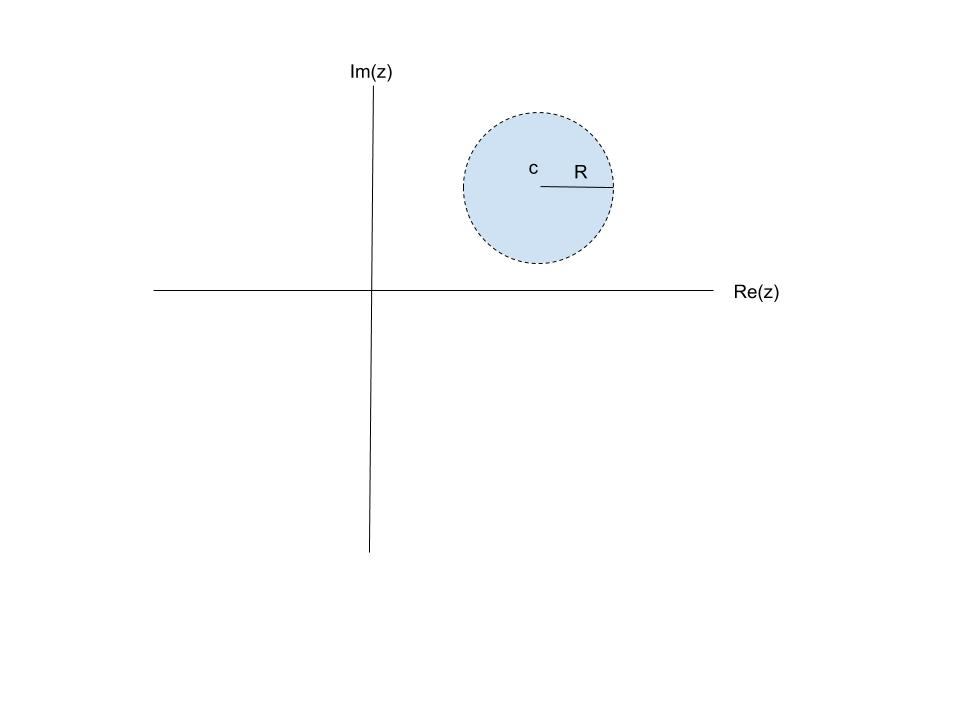
\includegraphics[width=0.75\columnwidth]{radiusConvergence}
	\end{figure}
	
	\noindent Some helpful facts... 
		\begin{itemize}
			\item $n^{1/n}\rightarrow 1$ as $n\rightarrow +\infty$
			\item $(1/n!)^{1/n}\rightarrow 0$ as $n\rightarrow +\infty$ 
		\end{itemize}
	
	
	\noindent\textit{Example} define $f(z) = \sum_{n=0}^{\infty}\frac{1}{n!}z^n$ then,\\ 
		\begin{align*}
			L &= \limsup (1/n!)^(1/n) = 0 \Rightarrow R = +\infty
		\end{align*}
	
	\noindent\textit{Example} define $\sum z^n$ then, 
		\begin{align*}
			L = \limsup 1^{1/n} = 1 \rightarrow R = 1/1 = 1
		\end{align*}
	\noindent Thus 
	the series converges absolutely for $|z|<1$. On this disc we have $\sum z^n = \frac{1}{1-z}$\\
	
	\noindent\textbf{Proof of theorem:} 
	\begin{proof}
		Assume $c=0$ and assume that $0<L<+\infty$ (other cases are dealt with similarly). (a) Assume $|z|<R$. We need to show that the series converges absolutely. From the assumption we have that $|z| < \frac{1}{L}$ which means that $L|z|<1$. Then let $\epsilon > 0$ such that $r:=(L+\epsilon)|z|<1$. By the definition of L we have that $|a_n|^{1/n} \leq L+\epsilon$ for large enough n. For the nth term of the series we have 
		\begin{align*}
			|a_n z^n| &= (|a_n|^{1/n}|z|)^n \\ 
				&\leq ((L+\epsilon)|z|)^n \\ 
				&= r^n 
		\end{align*}
		and $r<1$ so $\sum |a_nz^n|$ converges by comparison test ot the convergent geometric series $\sum r^n$ with $r<1$. \\ 
		
		\noindent If $|z|>R$ a similar argument show that the sequence of terms $a_nz^n$ do not even converge to zero and hence the series diverges. 
	\end{proof}
	

	\begin{theorem}
		Let $f(z) = \sum a_n (z-c)^n$ be a function defined by a power series with radius of convergence $0<R\leq\infty$ Then $f(z)$ is holomorphic in the disc $D_R(c)$, and has derivative	
			\begin{equation*}
				f'(z) = \sum\limits_{n=1}^\infty na_n(z-c)^{n-1}
			\end{equation*}
		\noindent Moreover, the radius of convergence for $f'(z)$ is also R. 
	\end{theorem}
	
	Once we show that all holomorphic functions are given by a power series than if we have $f(z)$ is once differentiable, it is infinitely differentiable. \\
	
	\textit{Example} $e^z = \sum \frac{1}{n!}z^n$ 
		\begin{align*}
			(e^z)' &= \sum_{n=1}^\infty n\frac{1}{n!}z^{n-1} \\ 
			\text{let } m &= n-1 \\ 
			 &= \sum_{m=0}^\infty \frac{1}{m!}z^m = e^z
		\end{align*}
	
\end{document}
































